\documentclass[smaller,pdf,svgnames]{beamer}

\title {A Genetic algorithm overview}
\author{Thomas Badie\\Victor Lenoir\\Pierre Parutto}
\institute{}

\usetheme{Warsaw}

%% To get the page numbering clean.
\defbeamertemplate*{footline}{shadow theme}
{%
  \leavevmode%
  \hbox{\begin{beamercolorbox}[wd=.5\paperwidth,ht=2.5ex,dp=1.125ex,leftskip=.3cm plus1fil,rightskip=.3cm]{author in head/foot}%
    \usebeamerfont{author in head/foot}\insertframenumber\,/\,\inserttotalframenumber\hfill\insertshortauthor
  \end{beamercolorbox}%
  \begin{beamercolorbox}[wd=.5\paperwidth,ht=2.5ex,dp=1.125ex,leftskip=.3cm,rightskip=.3cm plus1fil]{title in head/foot}%
    \usebeamerfont{title in head/foot}\insertshorttitle%
  \end{beamercolorbox}}%
  \vskip0pt%
}

% To do not have the summary on each slide.
\setbeamertemplate{headline}{}

\begin{document}

\begin{frame}
  \maketitle
\end{frame}

\begin{frame}{Table of contents}
  \tableofcontents
\end{frame}


\section{Theory}

\begin{frame}{Motivations}
  \begin{block}{Algorithmic problems}
    \begin{itemize}
      \item Stochastic
      \item Convergence
    \end{itemize}
  \end{block}

  \begin{block}{Modelisation problems}
    \begin{itemize}
      \item How to encode a problem?
      \item Size of the initial population?
      \item Mutation operator?
      \item Recombination operator?
      \item Individual selection?
    \end{itemize}
  \end{block}
\end{frame}

\subsection{Schemata Theorem}
\begin{frame}{Presentation}
  \begin{block}{Goal}
    \begin{itemize}
    \item Defined by J.Holland in 1975\cite{holland1992}.
    \item Represent a group of indidual who all share some caracteristics.
    \item One schema, two schemata ;)
    \end{itemize}
  \end{block}    

  \begin{block}{Definition}
    \begin{itemize}
    \item Defined on the alphabet: $\{0;1;\#\}$
    \item $\#$ is "Don't care": it can be 0 or 1
    \end{itemize}
  \end{block}
\end{frame}

\begin{frame}{Example and mesures}
  \begin{block}{Example}
    \begin{itemize}
    \item The schema: $H = 1\textcolor{red}{\#}10\textcolor{red}{\#}1\textcolor{red}{\#}$
    \item Represents the following individuals:
      \begin{center}
        $1\textcolor{red}{0}10\textcolor{red}{0}1\textcolor{red}{0}$,
        $1\textcolor{red}{0}10\textcolor{red}{0}1\textcolor{red}{1}$,
        $1\textcolor{red}{0}10\textcolor{red}{1}1\textcolor{red}{0}$,
        $1\textcolor{red}{0}10\textcolor{red}{1}1\textcolor{red}{1}$,
        $1\textcolor{red}{1}10\textcolor{red}{0}1\textcolor{red}{0}$,
        $\ldots$
      \end{center}
    \end{itemize}
  \end{block}

  \begin{block}{Measures}
    \begin{itemize}
      \item Order(o): number of fixed positions
      \item Defining length($\delta$): distance between the first and last defined positions.
      \item Here: $o(H) = 4$ and $\delta(H) = 5$
      \item Intuitively: schemata with low o and short $\delta$ have an higher probability of surviving from a generation to the next.
    \end{itemize}
  \end{block}
\end{frame}

\begin{frame}{Graphical representation}
  \begin{center}
    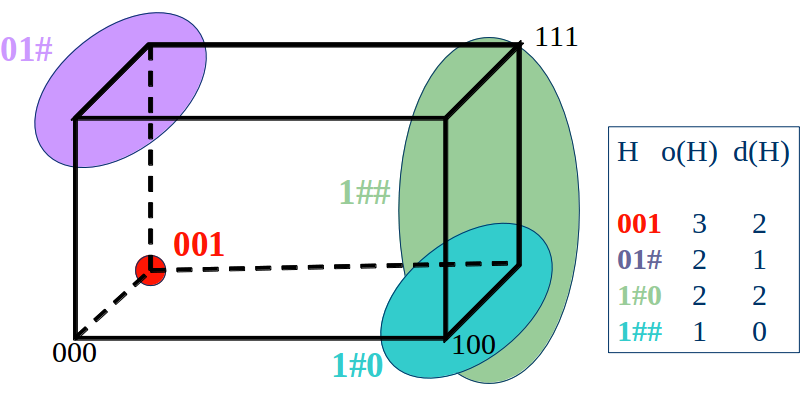
\includegraphics[scale=.4]{img/schema}
  \end{center}
\end{frame}

\begin{frame}{Possible evolutions : selection}
  \begin{block}{Hypothesis}
    \begin{itemize}
    \item Assume a fitness proportional reproduction
    \item $$\mathds{P}(x,t+1) = \frac{f(x)}{\bar{f(t)}}$$
    \end{itemize}
  \end{block}

  \begin{block}{Transmission of a schema}
    $$\begin{array}{lll}
      \mathds{P}(H,t+1) & = & \sum\limits_{x \in H} \frac{f(x)}{\bar{f(t)}}\\
      & = & m(H,t) \times \frac{f(H,t)}{\bar{f(t)}}\\
    \end{array}$$
  \end{block}
\end{frame}

\begin{frame}{Disruptions}
  \begin{block}{Mutation}
    \begin{itemize}
    \item bit-wise mutations with probability $p_m$
    \item Mutation events are independant
    \item $\mathds{P}_{Smuta}(H) \geq (1 - p_m)^{o(H)}$
    \end{itemize}
  \end{block}

  \begin{block}{Crossover}
    \begin{itemize}
      \item One point crossover with probability $p_c$
      \item l - 1 possible crossover points
      \item $\mathds{P}_{Scross}(H) \geq (1 - p_c \times \frac{\delta(H)}{l - 1})$
    \end{itemize}
  \end{block}
\end{frame}

\begin{frame}{Schema theorem}
  \begin{block}{Theorem}
    $$E(m(H,t+1)) \geq \underbrace{m(H,t) \times \frac{f(H,t)}{\bar{f(t)}}}_{\mathds{P}(x,t+1)}
    \underbrace{\times (1 - p_c \times \frac{\delta(H)}{l-1})\vphantom{\frac{f(H,t)}{\bar{f(t)}}}}_{\mathds{P}_{Smuta}}
    \underbrace{\times (1 - p_m)^{o(H)}\vphantom{\frac{f(H,t)}{\bar{f(t)}}}}_{\mathds{P}_{Scross}}$$
  \end{block}
\end{frame}

\begin{frame}{Extension to GP}
\end{frame}

\begin{frame}{Building Block hypothesis}
\end{frame}

\begin{frame}{Price's theorem}
\end{frame}

\begin{frame}{Limitations}
\end{frame}

\begin{frame}{Conclusion}
\end{frame}

\section{And in the real life?}
\begin{frame}
  \frametitle{And in the real life?}

  \begin{block}{Theory is good...}
    \begin{itemize}
    \item<1-2> To understand why it works.
    \item<2> Or why not.
    \end{itemize}
  \end{block}

  \visible<3-4> {

    \begin{block}{But what is is real power?}
      \begin{itemize}
      \item<3-4> Solve optimization problem.
      \item<4> Need to solve two problems: Encoding and Evaluation.
      \end{itemize}
    \end{block}
  }
\end{frame}




%%% Local Variables:
%%% mode: latex
%%% mode: flyspell
%%% TeX-master: "../genetic"
%%% ispell-dictionary: "en"
%%% compile-command: "cd .. && make"
%%% End:

\section{Application}

\subsection{Prerequisites}

\begin{frame}{MMORPG}
  \begin{block}{Definition}
    \begin{itemize}
    \item Massively Multiplayer Online RolePlaying Game
    \item Persistent World
    \end{itemize}
  \end{block}

  \begin{block}{Environment properties}
    \begin{itemize}
    \item Monsters
      \begin{itemize}
      \item Agressive
      \item Passive
      \end{itemize}
    \item

    \end{itemize}
  \end{block}

  \begin{block}{Purpose}
    \begin{itemize}
    \item Kill monsters
    \item Survive
    \end{itemize}
  \end{block}
\end{frame}

\begin{frame}{Openkore}

  \begin{block}{Definition}
    \begin{itemize}
    \item Program (Bot) which simulate a player in a MMORPG (here Ragnarok Online)
    \item Take a configuration file (so the bot is scriptable) as input
    \end{itemize}
  \end{block}

  \begin{block}{Why this application ?}
    \begin{itemize}
    \item There is a complex environment where the bot has life points, experience, position and a lot of other properties
    \item The bot is subjected to virtual physical constraints therefore we can have a lot of different fitness functions
    \item A lot of parameters available to customize the bot behaviour
    \item Easy to implement
    \end{itemize}
  \end{block}

\end{frame}
\subsection{Principle}

\begin{frame}{Parameters}

  \begin{block}{Parameters / Genes}
    \begin{itemize}
    \item The reaction of the bot when he sees an enemy:
      \begin{itemize}
      \item Attack
      \item Run away
      \item etc
      \end{itemize}
    \item A total of N * 6 parameters where N is the number of monsters on the map
    \end{itemize}
  \end{block}

  \begin{block}{Example}
    TODO: Display parameters for one bot
  \end{block}

\end{frame}

\begin{frame}{Repopulation}
  \begin{block}{Selected fitness functions}
    \begin{itemize}
    \item Life points : Try to minimize the life points lost in a round
    \item Experience points : Try to maximize the experience points acquired in a round
    \item Hybrid : Try to maximize the function $f = \frac{exp}{life} $
    \end{itemize}
  \end{block}

  \begin{block}{Selected reproduction}
    \begin{itemize}
    \item Mutation
    \item Crossover
    \end{itemize}
  \end{block}
\end{frame}

\subsection{Demonstration}

\begin{frame}{Demonstration}
  Demonstration !
\end{frame}

\subsection{Result}

\begin{frame}{Result}
  TODO: Insert results for different fitness functions here
\end{frame}



\begin{frame}
  \frametitle{Conclusion}
  Conclusion?
\end{frame}

\begin{frame}
  \frametitle{Questions?}
  % Thanks for your attention,

  % Questions?
  \begin{center}
    
\includegraphics[scale=0.7]{img/questions.jpg}
  \end{center}

\end{frame}

\section{References}

\begin{frame}{Bibliography}
  \footnotesize
  \bibliographystyle{unsrt}
  \bibliography{biblio}
\end{frame}

\end{document}
